\documentclass[letterpaper]{article}
%\documentclass[letterpaper,10pt]{scrartcl}

\usepackage[utf8]{inputenc}
\usepackage[pass,letterpaper]{geometry}
\usepackage{graphicx}

\title{Non-blocking,In-memory Database\thanks{Sponsor: Dr. Dechev}}
\author{Michael McGee, Robert Medina, Neil Moore, Jason Stavrinaky}
\date{9/18/2015}

\pdfinfo{%
  /Title    (Non-blocking, In-memory Database)
  /Author   (Michael McGee, Robert Medina, Neil Moore, Jason Stavrinaky)
  /Creator  (Neil Moore)
  /Producer ()
  /Subject  (Initial Project Description for COP4934)
  /Keywords ()
}

\begin{document}
  \pagenumbering{gobble}
  \maketitle
  \newpage
  \pagenumbering{arabic}

  \section{Introduction}
  This project's goal is to create a database that utilizes advanced multiprocessor techniques and algorithms to fully utilize modern hardware.
  We will be utilizing the Tervel framework that was developed by Dr. Dechev and his lab that implements multiprocessor-friendly memory management
  as well as various lock-free and wait-free data structures. These data structures will permit us to handle many concurrent transactions without 
  waits or locks.
  
  \subsection{Motivations}
  \subsubsection{Michael McGee's Motivation}
  My motivation for choosing this project is simply a desire to learn. I have always been interested in database systems as well concurrent programming. Nowhere do these issues more converge than in the project that Dr. Dechev proposed.  
  I hope to gain from this project, a greater understanding of the underlying principles of database system design, as well as discover broader applications for lock-free and wait-free data structures. I know that throughout the course of this project I will learn a great deal and come out as a much improved software developer and computer scientist.  
  \subsubsection{Robert Medina's Motivation}
  \textless Insert actual text here\textgreater
  \subsubsection{Neil Moore's Motivation}
  My motivation for working on this project is to further my knowledge on multiprocessor programming as well as high-performance computing.  
  As hardware vendors put more and more cores into computers, parallelization of algorithms and programs will become much more important than
  single-threaded performance. During my internship, I worked with both GPU compute (OpenCL) and virtualization technologies which exposed me
  to both multiprocessor and system programming. I really enjoyed working on those projects and I think this project will be the next step 
  in my progression as a software engineer and computer scientist.
  \subsubsection{Jason Stavrinaky's Motivation}
  I have always been interested in multiprocessor programming. Considering the future of programming is almost certainly heading towards a
  multiprocessor heavy paradigm, it is an essential skill. Working on a big project involving this is a great opportunity to learn. Not only
  about multiprocessor programming but also memory management. In addition, creating an open source solution to memSQL sounds like an exciting
  challange to undertake while also contributing to the programming community.
  \textless Insert actual text here\textgreater
  
  \section{Requirements}
  Our deliverable requirements are as follows:
  \begin{itemize}
   \item Able to run simple SQL benchmark such as the one bundled into SQLite.
   \item GitHub Page similar to the Tervel framework's.
   \item Source code on the UCF GitHub subdomain.
   \item In-depth documentation on project internals and architecture.
   \item Workshop paper that details new approaches used in database.
  \end{itemize}
  
  \section{Proposed Architecture}
  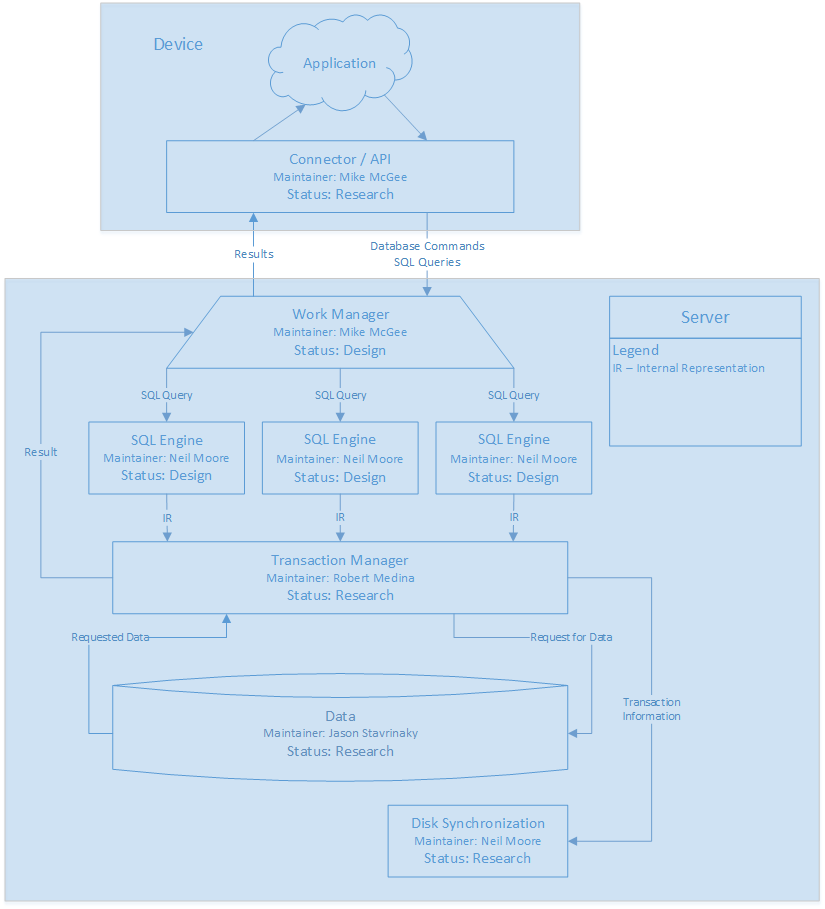
\includegraphics[scale=.5]{OpenMemDbDiagram.png}
  
  \section{Financial Concerns}
  Our sponsor is supplying us with a 64-core server that should be sufficient for our development needs. I do not believe any further financial
  support would be required.
  
  \section{Project Milestones}
  For this project we're going to utilize the incremental software development process which emphasizes development of small modules concurrently
  with a focus on:
  \begin{itemize}
   \item Communication to understand the objective
   \item Planning (process modeling, data flow)
   \item Development of program modules
   \item Integration and Deployment
  \end{itemize}
  \subsection{Milestone 1 - 10/30/2015}
  \begin{itemize}
   \item Initial documentation.
   \item Workshop paper motivation \& problem statement (half-page each).
   \item Workshop paper related work write-up with comparison to what this project attempts to do (half-page each).
   \item System architecture block diagram.
   \item Basic integration of Tervel into an application along with basic application framework.
  \end{itemize}
  \subsection{Milestone 2 - 12/15/2015}
  \begin{itemize}
   \item Connector implementation that can spawn threads upon SQL queries.
   \item Basic SQL engine that handles parsing and parameterization of queries.
   \item Initial design of API used by applications to access database.
  \end{itemize}
  \subsection{Milestone 3 01/30/2016}
  \begin{itemize}
   \item Finalized system architecture.
   \item Rudimentary implementation of the transaction manager.
   \item Preliminary implementation of the disk synchronization service.
   \item Further work on workshop paper
  \end{itemize}
  \subsection{Milestone 4 02/30/2016}
  \begin{itemize}
   \item 
  \end{itemize}






\end{document}
